\chapter{Phương pháp}

\section{Tập dữ liệu: Thử thách ISIC 2018}

Tập dữ liệu sử dụng trong nghiên cứu này là ISIC 2018 Skin Lesion Analysis Towards Melanoma Detection (Nhiệm vụ 3), chứa 10.015 ảnh dermoscopy phân bố trên bảy loại chẩn đoán.

\begin{table}[H]
\centering
\caption{Phân bố lớp của tập dữ liệu ISIC 2018.}
\label{tab:class_distribution_vn}
\begin{tabular}{llrrr}
\toprule
\textbf{Lớp} & \textbf{Tên đầy đủ} & \textbf{Train} & \textbf{Val} & \textbf{Test} \\
\midrule
NV    & Nốt ruồi sắc tố           & 4.693 & 1.006 & 1.006 \\
MEL   & Ung thư hắc tố             &   779 &   167 &   167 \\
BKL   & Dày sừng lành tính         &   769 &   165 &   165 \\
BCC   & Ung thư biểu mô tế bào đáy &   360 &    77 &    77 \\
AKIEC & Dày sừng quang hóa         &   229 &    49 &    49 \\
VASC  & Tổn thương mạch máu        &    99 &    21 &    22 \\
DF    & U xơ bì                    &    81 &    17 &    17 \\
\midrule
\textbf{Tổng} & & \textbf{7.010} & \textbf{1.502} & \textbf{1.503} \\
\bottomrule
\end{tabular}
\end{table}

NV chiếm 66,9\% mẫu huấn luyện; DF và VASC cộng lại chỉ chiếm 2,6\%, tỷ lệ 58:1. Tất cả thí nghiệm sử dụng phân chia phân tầng 70/15/15 giữ nguyên tỷ lệ các lớp.

\begin{figure}[H]
\centering
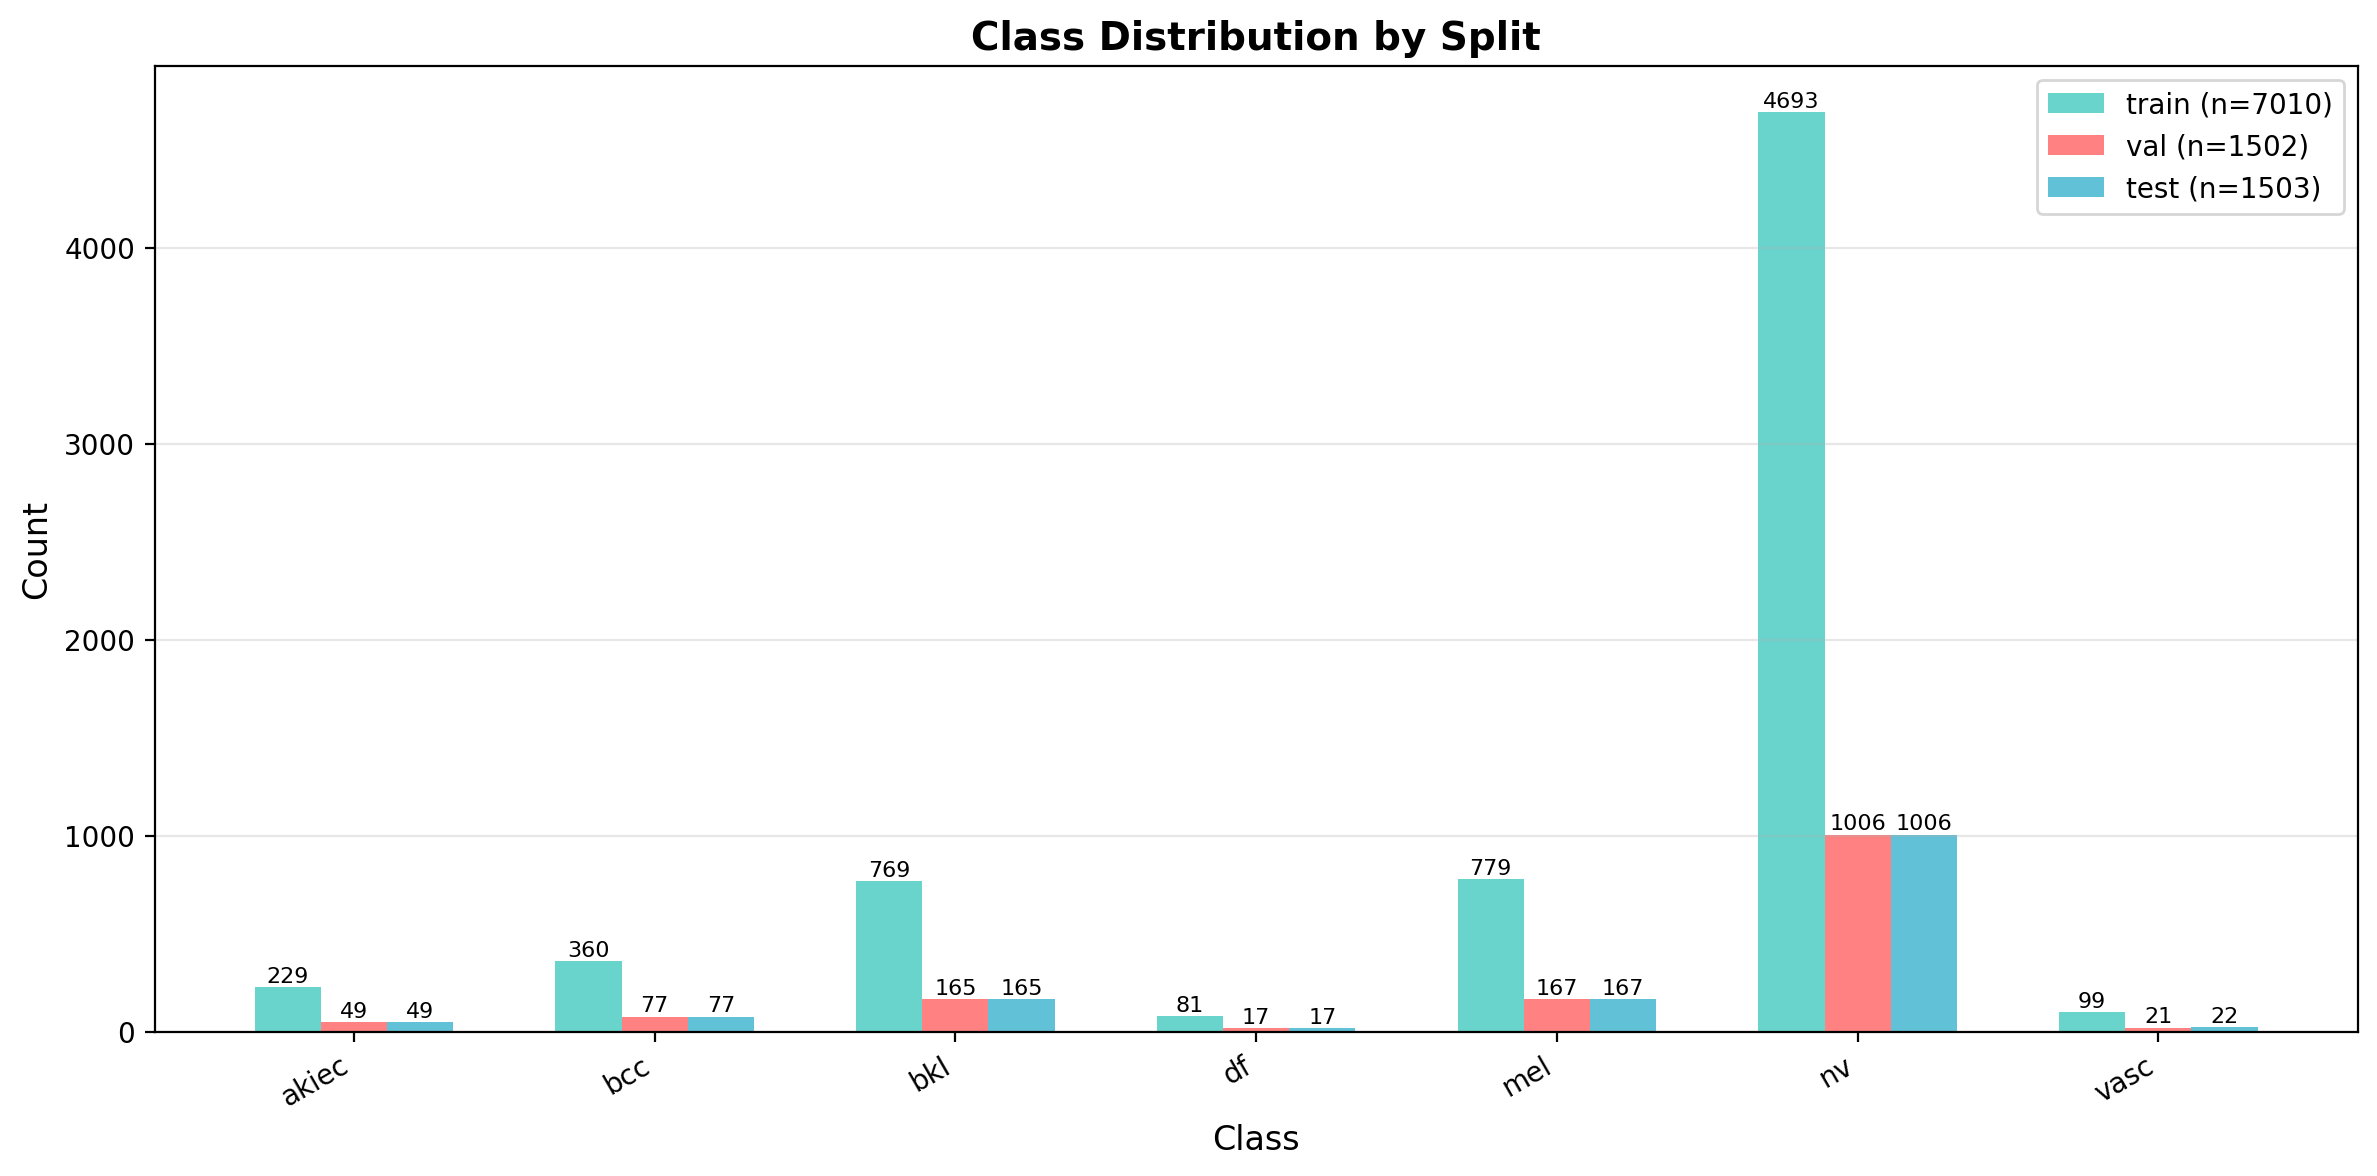
\includegraphics[width=\figwidth]{figures/class_distribution.png}
\caption{Phân bố lớp trên các tập huấn luyện, xác thực và kiểm tra. Sự mất cân bằng nghiêm trọng giữa NV và các lớp thiểu số (DF, VASC) thể hiện rõ ràng.}
\label{fig:class_distribution_vn}
\end{figure}

\section{Kiến trúc Mô hình}

Bốn kiến trúc được lựa chọn: ba CNN và một Vision Transformer. Tất cả được khởi tạo với trọng số ImageNet pretrained qua thư viện \texttt{timm} và được tinh chỉnh (fine-tune) trên ISIC 2018. Hình~\ref{fig:transfer_learning_vn} minh họa quy trình học chuyển giao này.

\begin{figure}[H]
\centering
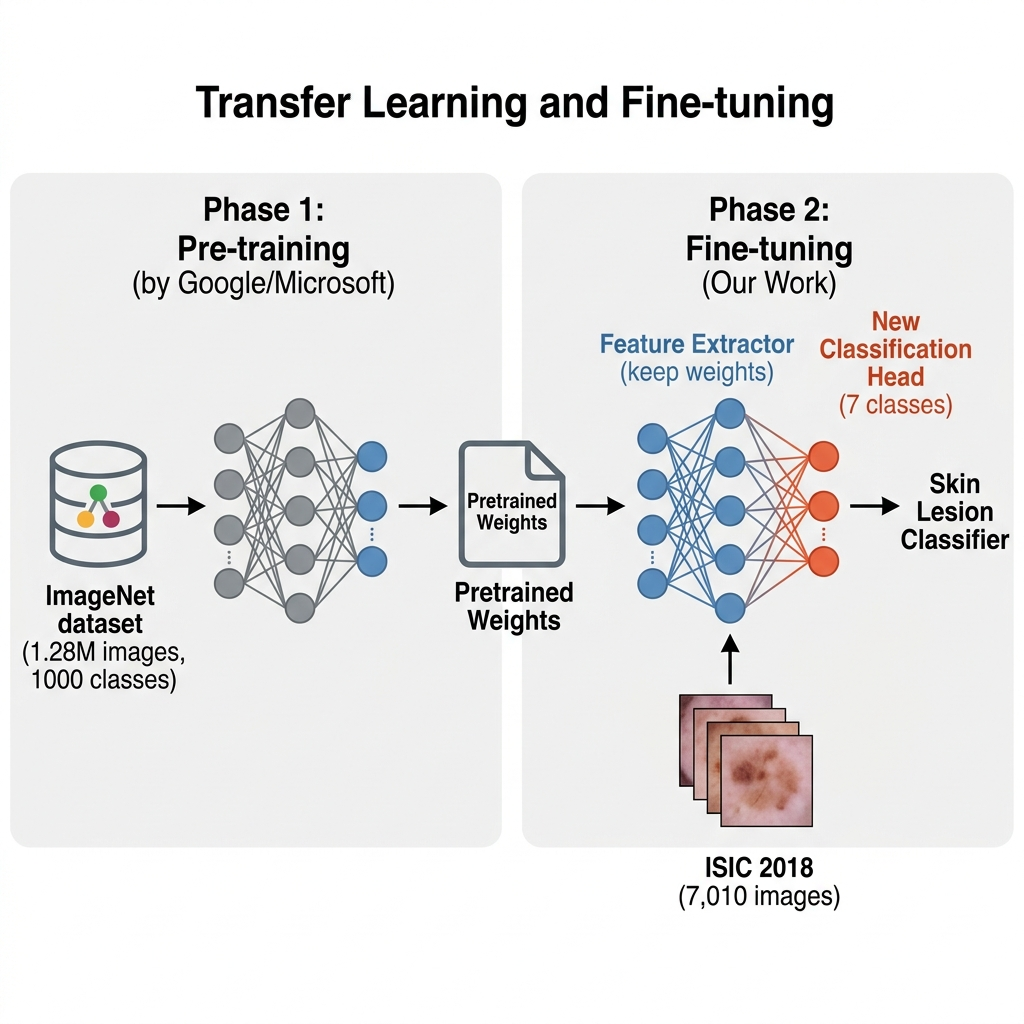
\includegraphics[width=\textwidth]{figures/transfer_learning.png}
\caption{Pipeline học chuyển giao: trọng số pretrained từ ImageNet được tải vào mỗi kiến trúc, đầu phân loại được thay thế để xuất 7 lớp tổn thương da, và toàn bộ mạng được tinh chỉnh trên tập ISIC 2018.}
\label{fig:transfer_learning_vn}
\end{figure}

\subsection{EfficientNet-B0}
Mô hình cơ sở của họ EfficientNet, thiết kế bằng Tìm kiếm Kiến trúc Thần kinh (NAS) và co giãn hỗn hợp (compound scaling). Với chỉ 5,3 triệu tham số, đạt độ chính xác cạnh tranh bằng cách tối ưu hóa đồng thời chiều sâu, chiều rộng và độ phân giải. Dropout ($p=0,3$) được thêm trước đầu phân loại.

\subsection{ResNet50}
50 lớp tổ chức thành bốn giai đoạn phần dư (residual stage). Kết nối tắt (skip connection) cho phép dòng gradient hiệu quả. 25,6 triệu tham số. Dropout ($p=0,3$).

\subsection{DenseNet121}
121 lớp với kết nối dày đặc: mỗi lớp nhận feature map được nối (concatenate) từ tất cả các lớp trước. Thúc đẩy tái sử dụng đặc trưng, giảm xuống khoảng 8 triệu tham số. Dropout ($p=0,25$).

\subsection{Swin-Tiny}
Vision Transformer phân cấp xử lý ảnh qua tự chú ý dựa trên cửa sổ dịch chuyển (shifted window). 28 triệu tham số. Tốc độ học thấp hơn ($1\times10^{-4}$), suy giảm trọng số cao hơn (0,05), warmup 5 epoch.

\begin{table}[H]
\centering
\caption{Tóm tắt bốn kiến trúc được đánh giá.}
\begin{tabular}{lrllr}
\toprule
\textbf{Mô hình} & \textbf{Tham số (M)} & \textbf{Loại} & \textbf{Đặc trưng chính} & \textbf{Dropout} \\
\midrule
EfficientNet-B0 & 5,3  & CNN & Co giãn hỗn hợp  & 0,30 \\
ResNet50        & 25,6 & CNN & Kết nối phần dư    & 0,30 \\
DenseNet121     & 8,0  & CNN & Kết nối dày đặc    & 0,25 \\
Swin-Tiny       & 28,0 & ViT & Chú ý cửa sổ dịch chuyển & 0,30 \\
\bottomrule
\end{tabular}
\end{table}

\section{Pipeline Huấn luyện}

Pipeline huấn luyện được xây dựng xung quanh một vấn đề trung tâm: mất cân bằng lớp 58:1. Bốn kỹ thuật giải quyết vấn đề này từ các góc độ khác nhau --- lấy mẫu, tăng cường dữ liệu, sửa đổi mục tiêu nhãn và điều chuẩn --- và các đóng góp cá nhân của chúng được định lượng trong nghiên cứu loại bỏ ở Chương~4. Hình~\ref{fig:training_pipeline_vn} cung cấp tổng quan toàn bộ pipeline.

\begin{figure}[H]
\centering
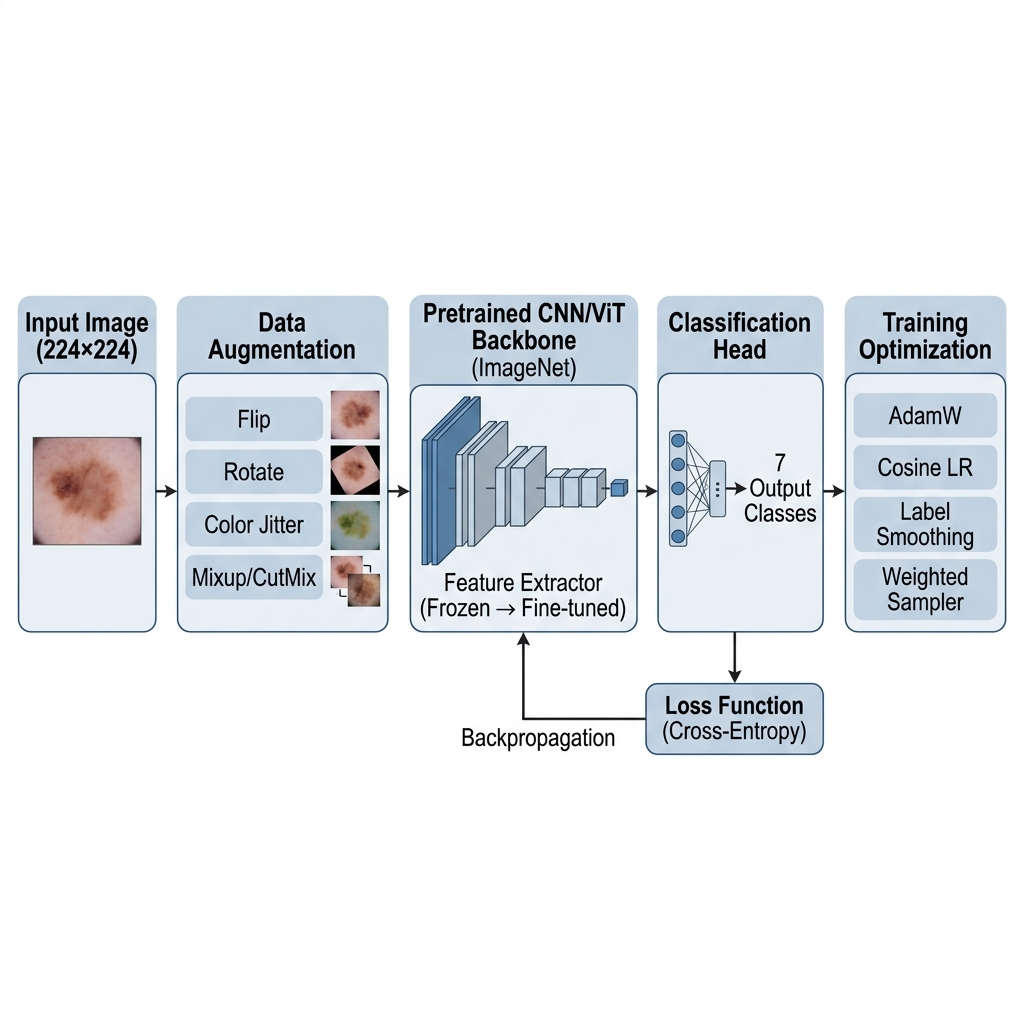
\includegraphics[width=\textwidth]{figures/training_pipeline.png}
\caption{Tổng quan pipeline huấn luyện. Ảnh đầu vào qua tăng cường dữ liệu (bao gồm Mixup/CutMix), đi qua backbone pretrained để trích xuất đặc trưng, và được phân loại bởi đầu ra. Pipeline được tối ưu với AdamW, lịch trình tốc độ học cosine, và làm mượt nhãn.}
\label{fig:training_pipeline_vn}
\end{figure}

\subsection{Lấy mẫu Ngẫu nhiên có Trọng số}

Để chống lại mất cân bằng lớp trong huấn luyện, một Weighted Random Sampler được sử dụng. Mỗi mẫu được gán một trọng số tỷ lệ nghịch với tần suất lớp của nó trong tập huấn luyện:
\begin{equation}
w_c = \frac{N}{C \cdot n_c}
\label{eq:class_weight_vn}
\end{equation}
trong đó $N$ là tổng số mẫu huấn luyện, $C$ là số lớp, và $n_c$ là số mẫu thuộc lớp $c$. Điều này đảm bảo các mini-batch xấp xỉ cân bằng lớp, ngăn mô hình phát triển thiên kiến về phía lớp đa số (NV).

\subsection{Tăng cường Mixup và CutMix}

Để điều chuẩn thêm và cải thiện tổng quát hóa, Mixup và CutMix được áp dụng với xác suất bằng nhau ($p = 0{,}5$ mỗi loại) trong huấn luyện.

\textbf{Mixup} tạo ra các ví dụ huấn luyện ảo bằng cách nội suy tuyến tính các cặp ảnh và nhãn của chúng:
\begin{equation}
\tilde{x} = \lambda x_i + (1 - \lambda) x_j, \quad \tilde{y} = \lambda y_i + (1 - \lambda) y_j
\end{equation}
với $\lambda \sim \text{Beta}(\alpha, \alpha)$ và $\alpha = 0{,}2$.

\textbf{CutMix} thay thế một vùng hình chữ nhật của một ảnh bằng vùng tương ứng từ một ảnh khác, điều chỉnh nhãn theo tỷ lệ diện tích của vùng:
\begin{equation}
\tilde{x} = M \odot x_i + (1 - M) \odot x_j, \quad \tilde{y} = \lambda y_i + (1 - \lambda) y_j
\end{equation}
trong đó $M$ là mask nhị phân chỉ vùng cắt và $\lambda$ bằng tỷ lệ vùng không bị che. CutMix alpha được đặt là 1,0.

Cả hai kỹ thuật buộc mô hình học từ các tín hiệu lai mơ hồ. Với chỉ 81 ảnh Dermatofibroma huấn luyện, huấn luyện cross-entropy thuần ghi nhớ các ví dụ đó trong vài epoch; Mixup và CutMix ngăn điều đó bằng cách đảm bảo không ví dụ huấn luyện nào có nhãn one-hot cứng.

\subsection{Làm mượt Nhãn (Label Smoothing)}

Nhãn one-hot tiêu chuẩn gán xác suất 1,0 cho lớp đúng và 0,0 cho mọi lớp khác. Label Smoothing phân phối lại một phần nhỏ khối lượng xác suất sang các lớp sai:
\begin{equation}
y_{\text{smooth}} = (1 - \epsilon) \cdot y_{\text{one-hot}} + \frac{\epsilon}{C}
\end{equation}
trong đó $\epsilon = 0{,}1$ là hệ số làm mượt và $C = 7$ là số lớp. Điều này ngăn mô hình gán xác suất 1,0 cho bất kỳ lớp nào, cải thiện calibration và, như ablation ở Chương~4 cho thấy, cải thiện Macro F1 --- mặc dù phải trả giá nhỏ về độ sắc nét AUC.

\subsection{Tối ưu hóa và Lập lịch}

Tất cả mô hình được huấn luyện với AdamW, vốn tách weight decay khỏi việc scale gradient thích nghi. Adam tiêu chuẩn hấp thụ weight decay vào các tốc độ học theo từng tham số, làm giảm hiệu lực điều chuẩn của nó; AdamW áp dụng weight decay như một hình phạt nhân tử cố định bất kể lịch sử gradient, dẫn đến tổng quát hóa tốt hơn trên dữ liệu giữ lại. Tốc độ học tuân theo lịch trình giảm cosine với khởi động tuyến tính:

\begin{itemize}
    \item \textbf{Pha khởi động} (3--5 epoch đầu): Tốc độ học tăng tuyến tính từ gần 0 lên giá trị mục tiêu. Điều này ngăn classification head được khởi tạo ngẫu nhiên tạo ra các gradient lớn làm bất ổn feature extractor pretrained trong vài cập nhật đầu.
    \item \textbf{Pha giảm cosine} (các epoch còn lại): Tốc độ học giảm theo đường cong cosine đến mức tối thiểu $1 \times 10^{-6}$, cho phép mô hình ổn định trong một vùng rộng, phẳng của loss landscape thay vì dao động quanh một minimum sắc.
\end{itemize}

\subsection{Tăng cường Dữ liệu}

Ngoài Mixup và CutMix, các phép tăng cường chuẩn sau được áp dụng trong huấn luyện:
\begin{itemize}
    \item Lật ngẫu nhiên ngang và dọc ($p = 0{,}5$)
    \item Xoay ngẫu nhiên (lên đến $\pm 90^\circ$)
    \item Color jittering (độ sáng, tương phản, độ bão hòa, hue; biên độ 0,25)
    \item Random Resized Crop (phạm vi scale: 0,85--1,0)
    \item Gaussian Blur ($p = 0{,}1$)
    \item Random Erasing ($p = 0{,}1$)
\end{itemize}

Mọi ảnh được resize về $224 \times 224$ và chuẩn hóa với mean và độ lệch chuẩn ImageNet. Batch size cố định 16 cho mọi mô hình. Giá trị này bị áp đặt bởi Swin-Tiny 28M tham số dưới huấn luyện mixed precision; giữ batch size giống nhau qua mọi kiến trúc đảm bảo bất kỳ khác biệt hiệu suất nào phản ánh chính các mô hình thay vì động lực tối ưu hóa.

\begin{table}[H]
\centering
\caption{Cấu hình siêu tham số cho từng mô hình.}
\begin{tabular}{lcccc}
\toprule
\textbf{Siêu tham số} & \textbf{EB0} & \textbf{RN50} & \textbf{DN121} & \textbf{Swin-T} \\
\midrule
Tốc độ học        & 3e-4  & 3e-4  & 2,5e-4 & 1e-4 \\
Suy giảm trọng số & 1e-3  & 1e-3  & 1e-3   & 5e-2 \\
Epoch khởi động   & 3     & 3     & 3      & 5 \\
Epoch tối đa      & 50    & 50    & 50     & 50 \\
Dừng sớm          & 12    & 12    & 12     & 12 \\
Mixup $\alpha$    & 0,2   & 0,2   & 0,2    & 0,2 \\
CutMix $\alpha$   & 1,0   & 1,0   & 1,0    & 1,0 \\
Làm mượt nhãn     & 0,1   & 0,1   & 0,1    & 0,1 \\
\bottomrule
\end{tabular}
\end{table}

\section{Các Chỉ số Đánh giá}

Accuracy một mình là chỉ số gây hiểu lầm ở đây: một bộ phân loại dự đoán Melanocytic Nevus cho mọi input đạt 67\% accuracy trong khi không phát hiện được gì có giá trị lâm sàng. Vì vậy các chỉ số sau được báo cáo song song với accuracy:

\begin{itemize}
    \item \textbf{Macro F1-Score.} Trung bình không trọng số của F1 theo lớp. Vì mỗi lớp đóng góp như nhau bất kể tần suất, một mô hình bỏ qua DF hoặc VASC bị phạt mạnh ngay cả khi accuracy tổng thể trông tốt. Đây là tiêu chí lựa chọn mô hình chính trong khóa luận này.
    \item \textbf{Weighted F1-Score.} F1 có trọng số theo cỡ lớp, đo độ chính xác tổng thể mà có tính tới mất cân bằng. Báo cáo cùng với Macro F1 cho bức tranh đầy đủ.
    \item \textbf{Macro AUC (One-vs-Rest).} Diện tích dưới đường cong ROC theo lớp, trung bình trên các lớp. AUC độc lập với ngưỡng quyết định và đo khả năng xếp hạng các trường hợp lớp dương trên các lớp âm. Trong triage lâm sàng nơi xác suất output được tiêu thụ trực tiếp để xếp hạng rủi ro, đây là chỉ số liên quan.
    \item \textbf{Cohen's Kappa ($\kappa$).} Độ đồng thuận đã hiệu chỉnh cho ngẫu nhiên. $\kappa > 0{,}6$ thường được xem là đồng thuận đáng kể.
    \item \textbf{Matthews Correlation Coefficient (MCC).} Tóm tắt toàn bộ ma trận nhầm lẫn (TP, TN, FP, FN) trong một con số duy nhất, đặc biệt phù hợp cho dữ liệu mất cân bằng vì không bị thiên kiến bởi lớp đa số.
    \item \textbf{Độ nhạy và Độ đặc hiệu theo lớp.} Độ nhạy (recall) = TP / (TP + FN); Độ đặc hiệu = TN / (TN + FP). Cả hai báo cáo theo lớp để định lượng riêng các hành vi gọi nhầm và bỏ sót.
\end{itemize}

\section{Chiến lược Kết hợp (Ensemble)}

Các phương pháp ensemble đã liên tục xuất hiện trong các bài nộp đạt kết quả cao nhất của ISIC challenge, và lý do thì đơn giản: các mô hình đa dạng phạm sai lầm ở các vị trí khác nhau, và việc lấy trung bình các output xác suất của chúng triệt tiêu một phần sai số đó. Khóa luận này sử dụng biểu quyết mềm (soft voting), lấy trung bình các vector xác suất thô trước khi lấy argmax. Hình~\ref{fig:ensemble_arch_vn} minh họa kiến trúc.

\begin{figure}[H]
\centering
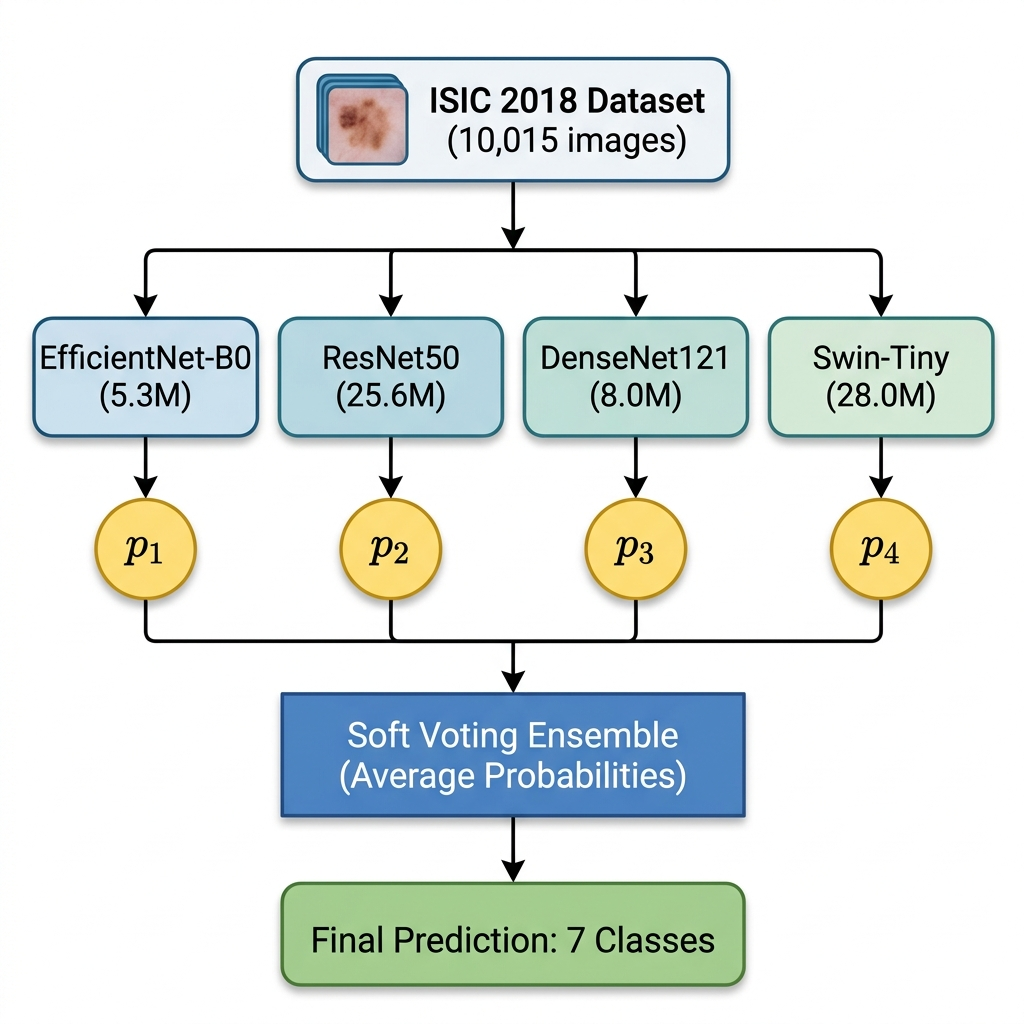
\includegraphics[width=\figwidth]{figures/ensemble_architecture.png}
\caption{Kiến trúc ensemble biểu quyết mềm. Mỗi trong bốn mô hình tạo một vector xác suất trên 7 lớp. Các vector được lấy trung bình theo từng phần tử, và lớp có xác suất trung bình cao nhất được chọn làm dự đoán cuối cùng.}
\label{fig:ensemble_arch_vn}
\end{figure}

Công thức formal:
\begin{equation}
\hat{y} = \arg\max_c \frac{1}{M} \sum_{m=1}^{M} p_m(c \mid x), \quad M = 4
\end{equation}

So với hard voting (mỗi mô hình lấy argmax rồi vote), soft voting giữ thông tin xác suất --- nó phân biệt được giữa ``cả bốn mô hình rất chắc MEL'' và ``hai mô hình vote MEL 51\%, hai mô hình vote NV 49\%''. So với stacking (meta-learner học trọng số ensemble), soft voting đơn giản hơn đáng kể, không cần val set thứ hai và không gây overfit thêm trên tập dữ liệu nhỏ.

\section{Khả năng Giải thích với Grad-CAM}

Sự chấp nhận lâm sàng của một công cụ chẩn đoán AI phụ thuộc vào nhiều hơn là độ chính xác --- một mô hình phải cung cấp lập luận có thể kiểm tra. Grad-CAM tính gradient của điểm số lớp mục tiêu $y^c$ đối với bản đồ đặc trưng tích chập cuối cùng $A^k$, và sử dụng các gradient đó để tạo bản đồ nhiệt không gian có trọng số theo kênh:
\begin{equation}
\alpha_k^c = \frac{1}{Z} \sum_i \sum_j \frac{\partial y^c}{\partial A_{ij}^k}, \quad L_{\text{Grad-CAM}}^c = \text{ReLU}\left(\sum_k \alpha_k^c A^k\right)
\end{equation}

Trong đó $\alpha_k^c$ là trọng số kênh thu được bằng global average pooling của gradient, và $L^c$ là heatmap đã ReLU (chỉ giữ phần đóng góp positive). Heatmap được up-sample về kích thước input gốc và overlay lên ảnh bằng colormap JET.

Đối với phân loại tổn thương da, Grad-CAM hoạt động như bài kiểm tra tính phản chứng: một mô hình tập trung activation vào nội thất và ranh giới tổn thương đang chú ý đến các đặc trưng mà bác sĩ nhận ra; một mô hình thắp sáng vạch ruler hoặc da nền thì không, bất kể accuracy trên test set là gì.
